\newpage
\section{Method} 

\subsection{The Data Handling and Devices}
The meteorological data was downloaded from the SMHI's website as CSV files. The data included hourly atmospheric pressure data, hourly rain data, and hourly wind data (speed and direction). Hourly aerosol data as \PM, measured over one-hour intervals, was also downloaded. Since the purpose of this thesis was to analyse aerosol concentrations in southern Sweden during high-pressure blocking events, one urban and one rural site were selected. The locations were chosen based on their classification as rural or urban and the length of time the stations had been in operation, where more data was considered better.  

\subsubsection{The Aerosol Data and Measurements}
The rural measuring station in the county of Skåne with the most aerosol data was Vavihill located in Svalöv, southern Sweden. This station was active from September 28, 1999, to November 15, 2017. However, due to missing data on some days, only \SI{57}{\%} of the period contained non-missing values. Additionally, between 2017 and 2018, the Vavihill station was relocated to nearby Hallahus, where it operated from May 10, 2018, to December 31, 2022, with \SI{93}{\%} of the period containing non-missing values. Combining these datasets resulted in a total of \SI{5371}{} days of hourly data. For an urban location in the county of Skåne, Malmö Rådhuset had the most data, with measurements recorded from June 3, 1999, to December 31, 2023. Here, \SI{90}{\%} of the recorded values were non-missing, resulting in \SI{8074}{} days of data. The geographical location of the two locations, together with pictures showing the surrounding area, can be seen in \autoref{fig:locations}.

The measurement device used at Vavihill was the ambient particulate monitor TEOM 1400. This monitor continuously collects airborne particles less than \SI{2.5}{\micro\meter} onto a filter and measures their mass using an oscillating microbalance technique \cite{thermofisherscientificinc.TEOMSeries1400a2007}. The oscillating microbalance works by vibrating at a natural frequency, which changes as particles accumulate on the filter. Since this frequency shift is proportional to the mass of the particles, their total mass can be calculated. The precision of the monitor was $\pm\SI{1.5}{\micro\gram\per\meter\cubed}$. Thus, the monitor provides high precision and stable measurements. However, a key limitation is that it cannot distinguish between different types of particles, as it only measures total mass. When the measuring station was moved to Hallahus, the measuring device was updated to the fine dust analysis system Palas FIDAS 200. This device works by an optical aerosol spectrometer, which samples particles from an isokinetic inlet through a polychromatic light-scattering channel where the scattering angles and intensities are measured. \cite{palasgmbhOperatingManualFidas}. This results in a high accuracy of $\pm\SI{0.1}{\micro\gram\per\meter\cubed}$, indicating an improvement from the previous device. 

The monitoring station in Malmö used several measuring devices over time, in conjunction with other equipment. Between the start of the monitoring and January 1, 2009, the TEOM 1400 monitor was used. From January 1, 2009, to December 31, 2015, the TEOM 1400, FDMS, and 8500 B or CB dryer were employed. Between January 1, 2016, and December 31, 2021, the TEOM 1405F and FDMS systems, along with the 8500 B, were in use. Finally, from January 1, 2022, the Palas FIDAS 200 monitor replaced the earlier systems. The FDMS (Filter Dynamics Measurement System) is a dynamic filter measurement system that enhances measurements by accounting for volatile and semi-volatile particles \cite{thermoscientific8500FDMSFilter2010}. The CB dryer and 8500 B are air dryers used to prevent moisture from entering the measurement devices, ensuring accurate data by avoiding interference caused by water vapour.

\begin{figure}[H]
    \centering
    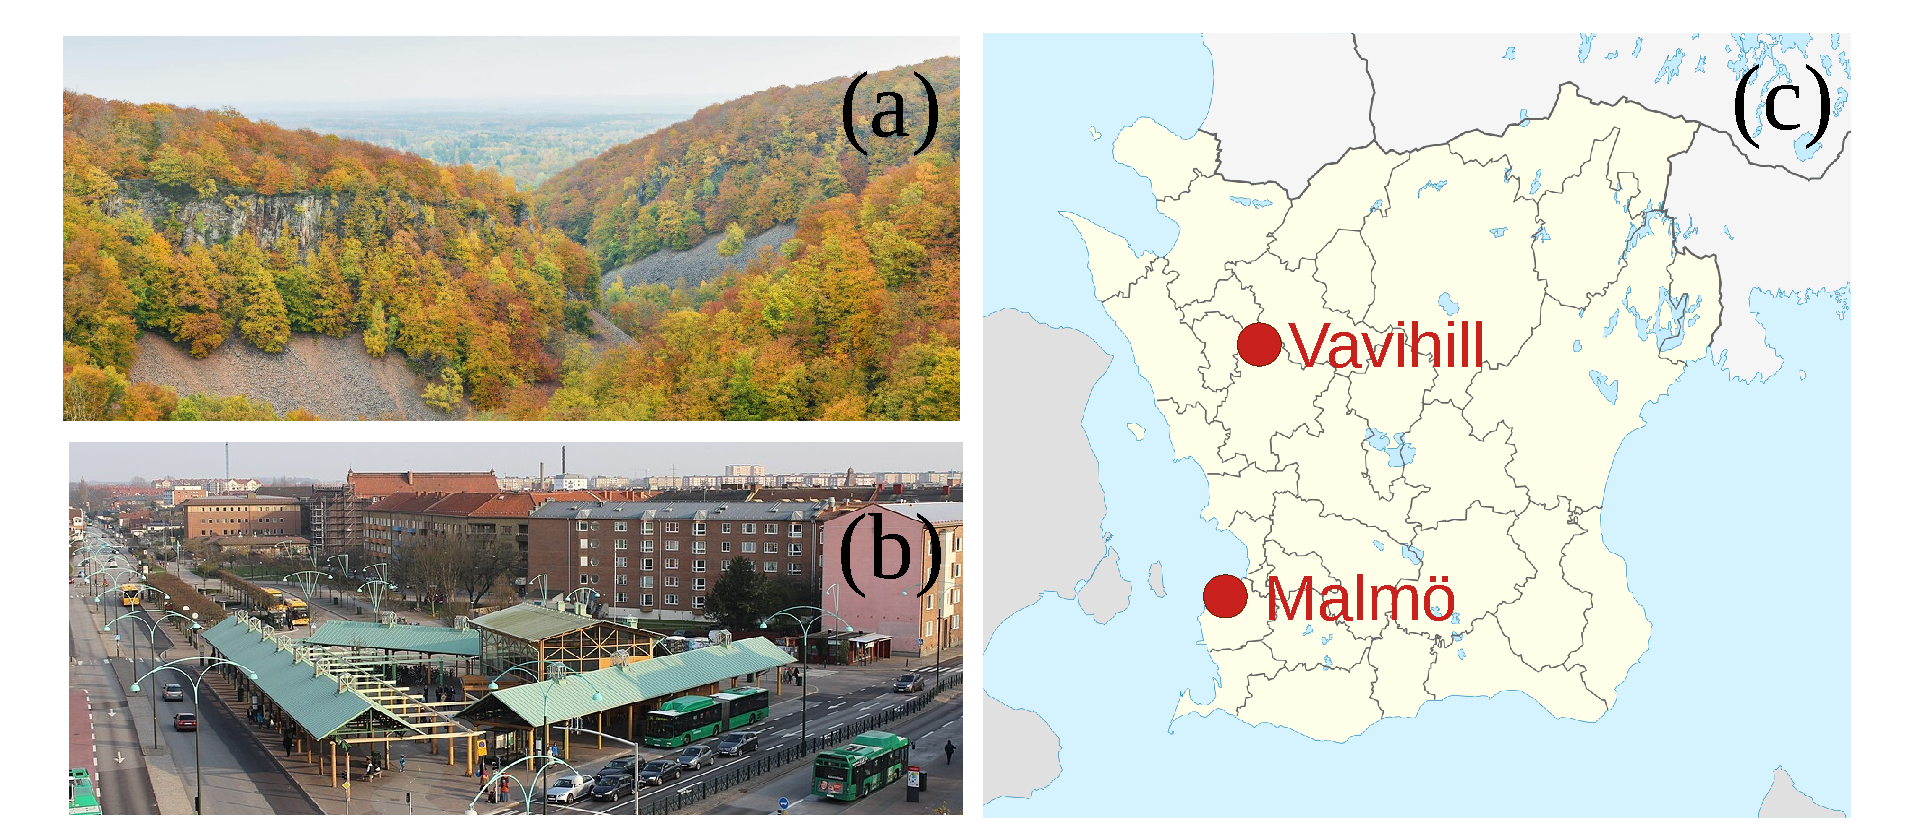
\includegraphics[width=0.7\textwidth]{Figures/Pictures.pdf}
    \caption{Pictures showing (a) the nearby national park, Söderåsen, to Vavihill \cite{s.perssonAutumnColorsSoderasen}, (b) a buss station in Malmö \cite{j.jonssonjulleSodervarnBusStation2015}, and (c) a map displaying the locations \cite{e.frohneLocationMapSkane2009}.  }
    \label{fig:locations}
\end{figure}


\subsubsection{The Meteorological Data and Measurements}
The meteorological data which was used in this thesis can be observed in \autoref{table:stations}. The time periods listed in the table show which periods was used this study, which may not represent the full operational range of the stations. Note that no particle data was collected from Ängelholm since this station was only used for detecting high-pressure blocking event during the last 74 years. The reason for not displaying wind data for Ängelholm was simply due to nun being available for this location. Also, the absence of device information in Ängelholm is due to airport security restrictions. Overall, the choice of locations was based on the proximity to the \PM measuring stations in the case for Vavihill and Malmö, and in the case of Ängelholm due to its proximity to the pressure measuring station. For Vavihill the wind and rain station had to be non coastal, since Vavihill is non coastal. This is because coastal regions can experience a daily cycles of sea breezes and land breezes, which alter the wind direction. Given that Ängelholm is situated \SI{44}{\km} from Vavihill and \SI{76}{\km} from Malmö, it is reasonable to question whether atmospheric pressure varies significantly over these distances. However, during the period from December 1, 1995, to October 1, 2024, the mean difference in pressure between Ängelholm and Helsingborg was $\SI{0.25\pm0.20}{\hecto\pascal}$, indicating minimal change. 

The PTB201A digital barometer operates using a silicon capacitive absolute pressure sensor, providing stable and accurate pressure values \cite{vaisalaPTB200DIGITAL1993}. The sensor functions by means of a flexed diaphragm inside a capacitor that bends in response to air pressure, causing a change in the capacitor's distance and thus a variation in the current. This device measures pressure in the range of \SI{600}{\hecto\pascal} to \SI{1100}{\hecto\pascal}, with an accuracy of $\pm\SI{0.3}{\hecto\pascal}$. Errors in the device may arise due to environmental factors, such as exposure to condensing gases. The Vaisala PTB220 digital barometer operates in a similar manner but offers a wider measurement range of \SI{500}{\hecto\pascal} to \SI{1100}{\hecto\pascal}, with an improved accuracy of $\pm\SI{0.15}{\hecto\pascal}$ \cite{vaisalaPTB220SeriesDigital2001}. The barometers used had been serviced every year or every other year.



The WAA15A anemometer works by a rotating chopper disc that interrupts an infrared beam, resulting in a laser pulse proportional to the wind speed \cite{vaisalaWindSetWA152021}. The WAV15A wind vane uses a counterbalanced vane with an optical disc. When the vane turns, infrared LEDs detect the change in angle with the disc and phototransistors, resulting in a precise measurement of the wind angle. he WAA15A anemometer measured wind speed with an accuracy of $\pm\SI{0.17}{\m\per\s}$, and the WAV15A wind vane measured the wind direction with an accuracy better than $\pm\ang{3}$. The wind instruments were serviced and calibrated every year or every other year, and had been in use since 1995. Like the wind monitor, the Geonor T200 rain monitor had been serviced and calibrated every year or every other year. This device works by measuring precipitation with a vibrating wire sensor that detects weight changes from the water droplets \cite{geonorinc.T200BSeriesAll2019}. The device has a measurement accuracy better than $\pm\SI{0.1}{\mm}$. 


\begin{table}[h]
    \centering
    \caption{The meteorological data for each location.}
\renewcommand{\arraystretch}{1.45} % Larger vertical spacing
\begin{tabular}{ll|l|l|l|}
\cline{3-5}
 &
   &
  \textbf{Vavihill} &
  \textbf{Malmö} &
  \textbf{Ängelholm} \\ \hline
\multicolumn{1}{|l|}{\textbf{\begin{tabular}[c]{@{}l@{}}Air\\ pressure\end{tabular}}} &
  Station &
  \begin{tabular}[c]{@{}l@{}}Helsingborg (25 km away \\ from particle monitor)\end{tabular} &
  \begin{tabular}[c]{@{}l@{}}Helsingborg (49 km away \\ from particle monitor)\end{tabular} &
  Ängelholm airport \\ \cline{2-5} 
\multicolumn{1}{|l|}{} &
  Period &
  \begin{tabular}[c]{@{}l@{}}August 2, 1995 \\ to October 10, 2024.\end{tabular} &
  \begin{tabular}[c]{@{}l@{}}August 2, 1995 \\ to October 10, 2024.\end{tabular} &
  \begin{tabular}[c]{@{}l@{}}January 5, 1946 \\ to October 1, 2024\end{tabular} \\ \cline{2-5} 
\multicolumn{1}{|l|}{} &
  Device &
  \begin{tabular}[c]{@{}l@{}}Vaisala PTB220 \\ (April 15, 2015,  to April 17, \\ 2025, and from September \\ 19, 2004, to May 23, 2014)\\ PTB201A (Remaining time)\end{tabular} &
  \begin{tabular}[c]{@{}l@{}}Vaisala PTB220  \\ (April 15, 2015,  to April 17, \\ 2025, and from September \\ 19, 2004, to May 23, 2014)\\ PTB201A (Remaining time)\end{tabular} &
  No info \\ \hline
\multicolumn{1}{|l|}{\textbf{Wind}} &
  Station &
  \begin{tabular}[c]{@{}l@{}}Hörby (35 km away from \\ particle monitor)\end{tabular} &
  \begin{tabular}[c]{@{}l@{}}Malmö (6 km away from \\ particle monitor)\end{tabular} &
  \multicolumn{1}{c|}{-} \\ \cline{2-5} 
\multicolumn{1}{|l|}{} &
  Period &
  \begin{tabular}[c]{@{}l@{}}August 1, 1995, to October \\ 1, 2020.\end{tabular} &
  \begin{tabular}[c]{@{}l@{}}January 1, 1990, to \\ December 31 2020.\end{tabular} &
  \multicolumn{1}{c|}{-} \\ \cline{2-5} 
\multicolumn{1}{|l|}{} &
  Device &
  \begin{tabular}[c]{@{}l@{}}Vaisala WAA15A (speed)\\ Vaisala WAV15A (direction)\end{tabular} &
  \begin{tabular}[c]{@{}l@{}}Vaisala WAA15A (speed)\\ Vaisala WAV15A (direction)\end{tabular} &
  \multicolumn{1}{c|}{-} \\ \hline
\multicolumn{1}{|l|}{\textbf{Rain}} &
  Station &
  \begin{tabular}[c]{@{}l@{}}Hörby (35 km away from \\ particle monitor)\end{tabular} &
  \begin{tabular}[c]{@{}l@{}}Malmö (6 km away from \\ particle monitor)\end{tabular} &
  Ängelholm and Tånga. \\ \cline{2-5} 
\multicolumn{1}{|l|}{} &
  Period &
  \begin{tabular}[c]{@{}l@{}}August 1, 1995, to October \\ 1, 2020.\end{tabular} &
  \begin{tabular}[c]{@{}l@{}}November 21, 1995, to \\ December 31 2020.\end{tabular} &
  \begin{tabular}[c]{@{}l@{}}January 18, 1947, to \\ November 30, 2001 \\ and December 19, 1973 \\ to August 31, 2024.\end{tabular} \\ \cline{2-5} 
\multicolumn{1}{|l|}{} &
  Device &
  Geonor T200 &
  Geonor T200 &
  No info and beaker. \\ \hline
\end{tabular}
    \label{table:stations}
\end{table}

\newpage

\subsection{The Identification of High-Pressure Blocking Events}
To evaluate the occurrence of high-pressure blocking event for Vavihill or Malmö, the rain data and atmospheric air pressure were used, which can be seen in \autoref{fig:definiton}. For a period to be defined as a high-pressure event, the atmospheric pressure had to be over \SI{1014}{\hecto\pascal}, and the rainfall had to be less than \SI{0.5}{\mm\per\hour}. These values were based on the fact that \SI{1014}{\hecto\pascal} was the mean atmospheric pressure from Helsingborg, and \SI{0.5}{\mm\per\hour} was chosen since this is considered as very light rain. Since a high-pressure blocking event covers a large geographical area, and Vavihill and Malmö are located close to each other, a blocking event observed at one location should also be detectable at the other. To account for this, all identified high-pressure blocking events at one location were required to correspond to an event at the other location within a maximum time difference of \SI{5}{\hour}. However since Vavihill and Malmö used the same air pressure measuring station, this meant that the precipitation in both locations had to be under \SI{0.5}{\mm\per\hour} for the event. For a high-pressure event to be considered a high-pressure blocking event, the criteria for a high-pressure event had to persist for at least \SI{120}{\hour} (5 days). This value was chosen since a 5-day limit is often considered when classifying high-pressure blocking events \cite{lupoAtmosphericBlockingEvents2020}.

The rain-limit was set to \SI{2}{\mm\per\day} in Ängelholm since daily precipitation measured used instead. This value was chosen since it corresponds to a small amount of rainfall for a day, and almost no rainfall should be observed during high-pressure blocking events. The choice of \SI{0.5}{\mm\per\hour} for hourly data is motivated by the fact that continuous light rain over a 24-hour period is very rare. As a result, daily precipitation levels seldom reach \SI{12}{\mm\per\day}, and are more commonly around \SI{2}{\mm\per\day}.  


\vspace{1cm}

\begin{figure}[H]
    \centering
    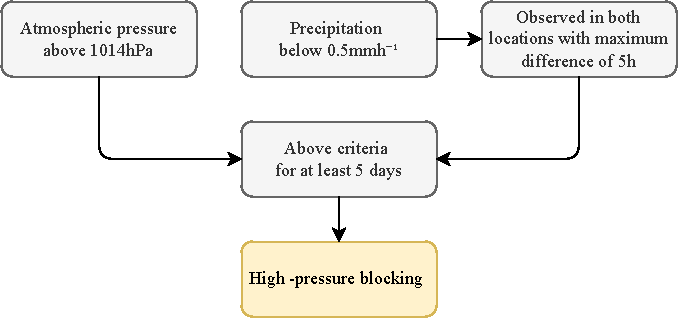
\includegraphics[width=0.7\textwidth]{Figures/Graph_BcThesis.pdf}
    \caption{This figure show how a high-pressure blocking events was defined in Vavihill and Malmö.}
    \label{fig:definiton}
\end{figure}

\newpage


\subsection{The Data Analysis}
The evolution of \PM during the high-pressure blocking events were evaluated by calculating the mean and standard deviation of \PM for each hour of all the high-pressure blocking events, to evaluate the average progression of aerosols over time. This was done using the Python packages \texttt{NumPy} and \texttt{pandas}. Since the high-pressure blocking events varied in length, a minimum of eight events was required when calculating the mean and standard deviation on the \PM data. The mean \PM value was then compared with the mean \PM value during periods without high-pressure blocking events, as well as with the EU annual mean limit for \PM. Due to the lack of \PM data during some high-pressure blocking events, a filter was applied, stating that a period needed \SI{85}{\%} \PM coverage in order to be analysed.

To evaluate if the \PM levels returned to normal after the end of the events, the mean and standard deviation were also calculated from the end onwards. This clarified whether an increase was observed and whether it corresponded to the high-pressure blocking event or not. Furthermore, if elevated levels were observed, this helped evaluate how quickly the levels returned to normal.

The data was sorted in different ways to explore how the \PM concentration depended on different parameters. Firstly, the data was sorted into one of four wind categories: northeast (310° to 70°), southeast (70° to 190°), west (190° to 310°), and no specific direction. This was done by categorizing the data if \SI{60}{\%} of the wind directional data fell into one of these categories, with zero wind speed being handled as a missing value.

Secondly, the data was sorted based on the season of the blocking. This was evaluated by taking the midpoint date of the blocking and categorizing the season by the month it occupied. December, January, and February were considered winter; March, April, and May were considered spring; June, July, and August were considered summer and September, October, and November were considered autumn. Lastly, the data was categorized based on the strength of the high-pressure blocking, where a weak high-pressure blocking event had a mean atmospheric pressure between \SI{1014}{\hecto\pascal} and \SI{1020}{\hecto\pascal}, an medium strong event had a mean atmospheric pressure between \SI{1020}{\hecto\pascal} and \SI{1025}{\hecto\pascal}, and an stronger event had a mean atmospheric pressure over \SI{1025}{\hecto\pascal}.

The last task of this study was to evaluate whether high-pressure blocking events had become increasingly more common. This was evaluated in two different ways: by calculating the number of days under high-pressure blocking events per year, and the number and lengths of high-pressure blocking events per year. The number of days of blocking was also sorted by the season of the blocking to provide more insight into the nature of the high-pressure blocking events. 

\newpage
\subsection{Statistical Evaluation: The Mann-Kendall Test and Sen's Slope}
To evaluate statistical significance of the trends found in the study, the statistical Mann-Kendall test was used. The Mann-Kendall test was applied to evaluate whether the \PM mean during high-pressure blocking events had increased, and if so, by how much. The Mann-Kendall test is a non-parametric statistical test used to calculate the monotonic trend and the significance of the result of a dataset. This test is commonly used in climate physics due to the challenges posed by many parameters and complex distributions. The test works by calculating the difference between each time step in the dataset. The output will be a p-value below 0.05 if the test provides a significant result, meaning that the trend is unlikely to be caused by randomness. Kendall's $\tau$-value is used to evaluate the monotonic increase of the dataset, where -1 indicates a total monotonic decrease, 1 indicates a total monotonic increase, and 0 indicates no monotonic trend. The $\tau$-value can be summarized by the formula 
\begin{equation}
    \tau = \frac{C - D}{C + D,}
    \label{eq:Kendalltau}
\end{equation}
where $C$ is the number of concordant pairs and $D$ is the number of discordant pairs. A Concordant pair is when two neighbouring data points increase with the time step, and discordant pair decreases with the time step. If the result yielded a $\tau$-value above 0.5, the result was labelled as a clear increase. 

Sen's slope is a method, often used together with the Mann-Kendall test, of performing linear regression on the data. If a monotonic increase is shown by the Mann-Kendall $\tau$, Sen's slope provides an estimate of the magnitude of that increase. The method differs from the least squares method because it uses the median to calculate the slope. This ensures that outliers, which are common in weather data, do not affect the results. Sen's slope is calculated as 
\begin{equation}
    S_{i} = \frac{\rho_{i+1} - \rho_i}{t_{i+1} - t_i} \quad \text{Sen's slope} = \text{median}(S_{i}),
    \label{eq:Senslope}
\end{equation}
where $i$ represents the indices, $\rho$ represents the concentration of \PM, and $t$ represents time. The program used for the Mann-Kendall test was the \texttt{pymannkendall} package in Python \cite{hussainmd.PyMannKendallPythonPackage2019}.
